\begin{outline-text-1}
\begin{center}
浅井 政太郎

東京大学大学院 総合文化研究科 福永研究室 D2
\end{center}
\end{outline-text-1}

\section{注意}
\label{sec-1}

今日の発表はいろいろなヒトの発表を借りて切り貼りしています

\begin{itemize}
\item 『フカシギの数え方』 おねえさんといっしょ! みんなで数えてみよう!
\item ZDD とフロンティア法 2017年版 ver 0.1 奈良先端科学技術大学院大学 川原 純
\item ZDDを用いたパスの列挙と索引生成 川原 純 (JST ERATO 研究員)
\item ICAPS2012-Tutorial Decision Diagrams in Discrete and Continuous Planning (Scott Sanner)
\item AAAI2016-Tutorial  Symbolic Methods for Probabilistic Inference, Optimization, and Decision-making (Scott Sanner)
\item ICAPS2016-Tutorial Decision Diagrams for Discrete Optimization (John Hooker CMU)
\end{itemize}

\section[Decision Diagram とは]{Decision Diagram とは\hfill{}\textsc{4min}}
\label{sec-2}

「『フカシギの数え方』 おねえさんといっしょ! みんなで数えてみよう!」で紹介されないデータ構造

二倍速で見ましょう

\section{今日のお話}
\label{sec-3}

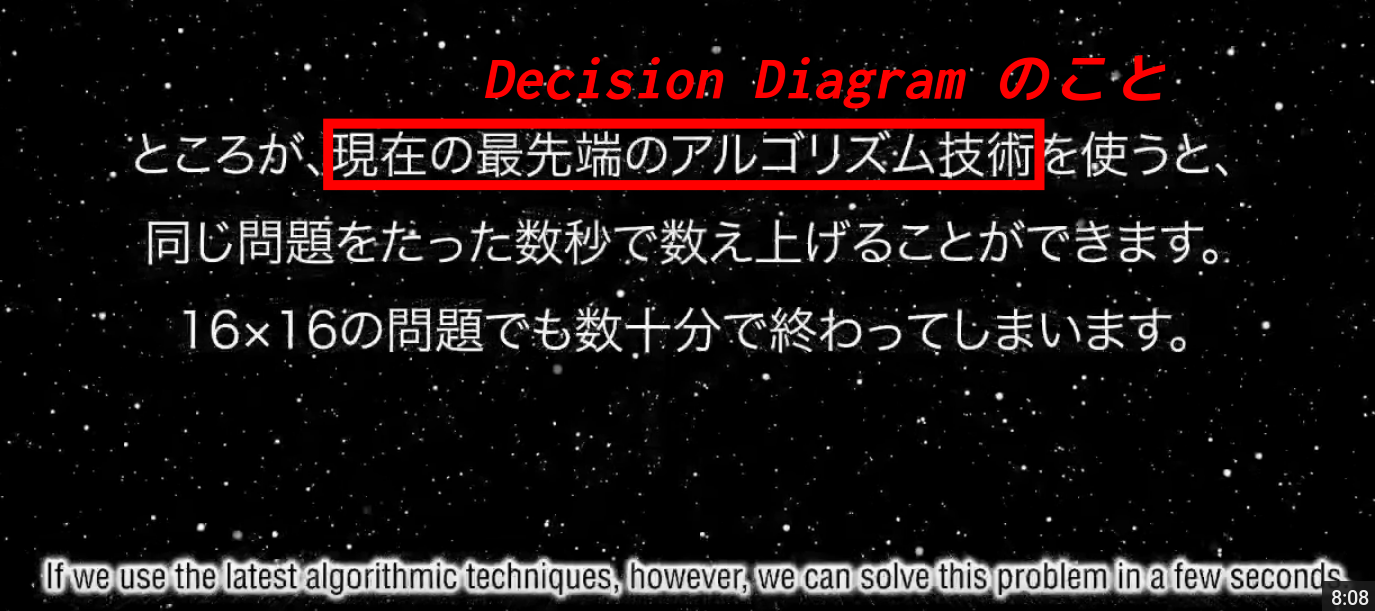
\includegraphics{img/static/latest-tech.png}

\begin{itemize}
\item これをCLから扱うライブラリを紹介
\end{itemize}

\section{Decision Diagrams (DDs)}
\label{sec-4}

\begin{container-fluid}
\begin{row-fluid}
\begin{span6}
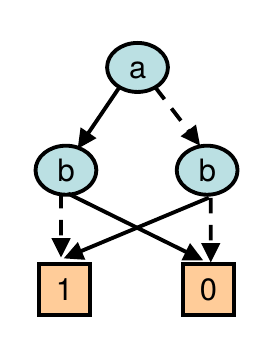
\includegraphics{img/static/dd.png}
\end{span6}
\begin{span6}
\begin{itemize}
\item 決定木(Decision Tree) のグラフ版
\item 関数をコンパクトに表現できる:
\begin{itemize}
\item $B = \{0, 1\}$
\item $f: B^n \rightarrow B$ : BDD,ZDD
\item $f: B^n \rightarrow R$ も可能 (ADD)
\end{itemize}
\end{itemize}
\end{span6}
\end{row-fluid}
\end{container-fluid}

\subsection{XOR関数を線形サイズで保持できる}
\label{sec-4-1}

Treeでは指数サイズのノードが必要。

AND と OR は DDでもTreeでも線形。

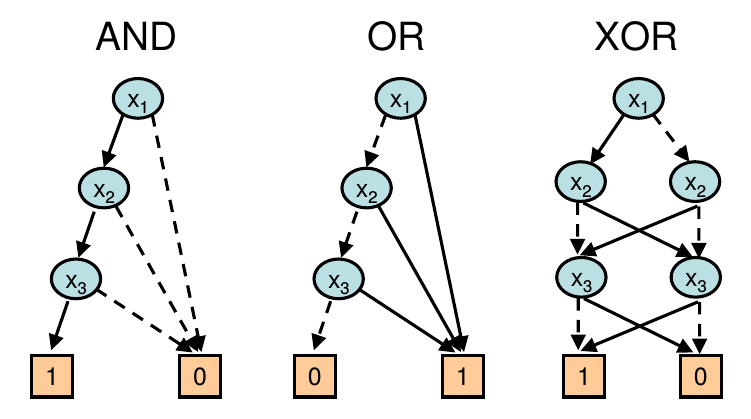
\includegraphics{img/static/dd-xor.png}

\subsection{Boolean Function を表現してみる (真理値表)}
\label{sec-4-2}

\begin{container-fluid}
\begin{row-fluid}
\begin{span6}
\begin{center}
\begin{tabular}{|ccc|c|}
$a$ & $b$ & $c$ & $F(a,b,c)$\\
\hline
0 & 0 & 0 & 0\\
0 & 0 & 1 & 0\\
0 & 1 & 0 & 0\\
0 & 1 & 1 & 1\\
1 & 0 & 0 & 0\\
1 & 0 & 1 & 1\\
1 & 1 & 0 & 0\\
1 & 1 & 1 & 1\\
\end{tabular}
\end{center}
\end{span6}
\begin{span6}
\begin{itemize}
\item 真理値表を使えば出来る
\item 動くけど、もっとコンパクトに出来る
\end{itemize}
\end{span6}
\end{row-fluid}
\end{container-fluid}

\subsection{Boolean Function を表現してみる (木/Decision Tree)}
\label{sec-4-3}

ノードごとにTrue/Falseかで進む枝が決まる

表よりコンパクト

\begin{container-fluid}
\begin{row-fluid}
\begin{span8}
\begin{center}
\begin{tabular}{|ccc|c|}
$a$ & $b$ & $c$ & $F(a,b,c)$\\
\hline
0 & 0 & 0 & 0\\
0 & 0 & 1 & 0\\
0 & 1 & 0 & 0\\
0 & 1 & 1 & 1\\
1 & 0 & 0 & 0\\
1 & 0 & 1 & 1\\
1 & 1 & 0 & 0\\
1 & 1 & 1 & 1\\
\end{tabular}
\end{center}
\end{span8}
\begin{span4}
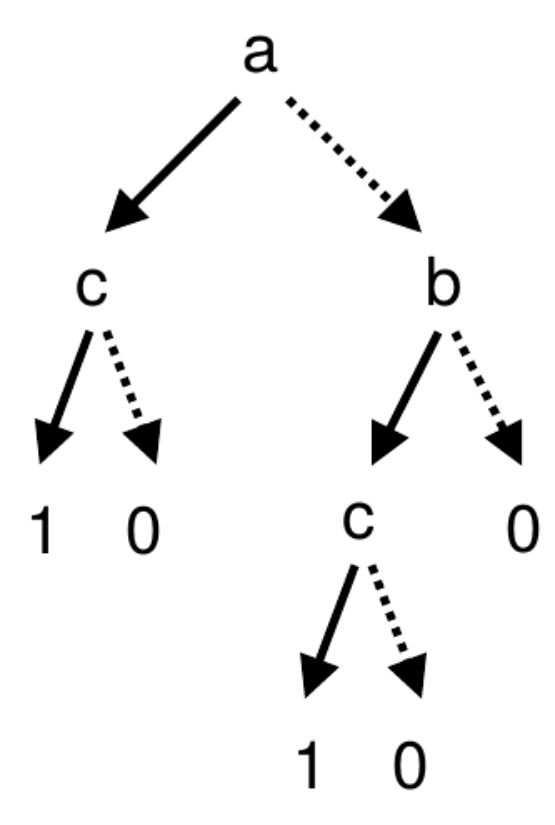
\includegraphics{img/dd-tree.png}
\end{span4}
\end{row-fluid}
\end{container-fluid}

\subsection{Boolean Function を表現してみる (木/Decision Tree)}
\label{sec-4-4}

でもまだ無駄な重複がある

\begin{container-fluid}
\begin{row-fluid}
\begin{span8}
\begin{center}
\begin{tabular}{|ccc|c|}
$a$ & $b$ & $c$ & $F(a,b,c)$\\
\hline
0 & 0 & 0 & 0\\
0 & 0 & 1 & 0\\
0 & 1 & 0 & 0\\
0 & 1 & 1 & 1\\
1 & 0 & 0 & 0\\
1 & 0 & 1 & 1\\
1 & 1 & 0 & 0\\
1 & 1 & 1 & 1\\
\end{tabular}
\end{center}
\end{span8}
\begin{span4}
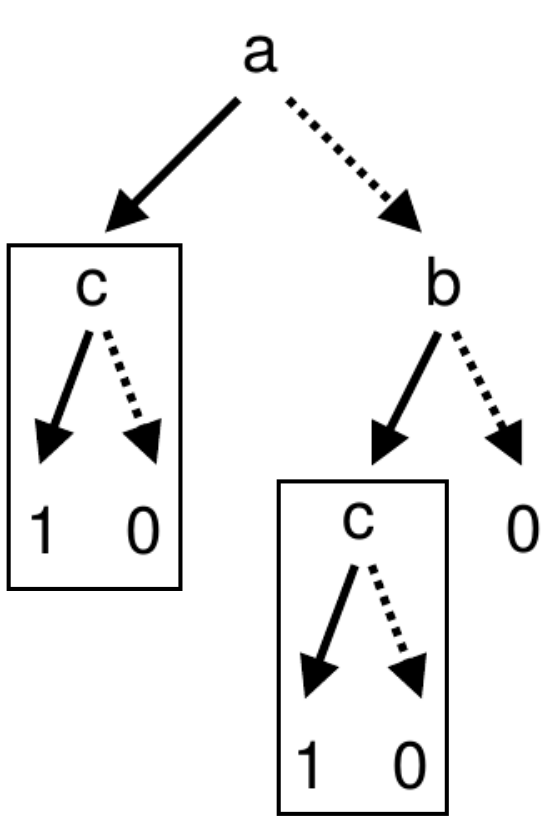
\includegraphics{img/dd-tree2.png}
\end{span4}
\end{row-fluid}
\end{container-fluid}

\subsection{Boolean Function を表現してみる (グラフ/Decision Diagram)}
\label{sec-4-5}

重複を共有してグラフにしよう!

\begin{container-fluid}
\begin{row-fluid}
\begin{span9}
\begin{center}
\begin{tabular}{|ccc|c|}
$a$ & $b$ & $c$ & $F(a,b,c)$\\
\hline
0 & 0 & 0 & 0\\
0 & 0 & 1 & 0\\
0 & 1 & 0 & 0\\
0 & 1 & 1 & 1\\
1 & 0 & 0 & 0\\
1 & 0 & 1 & 1\\
1 & 1 & 0 & 0\\
1 & 1 & 1 & 1\\
\end{tabular}
\end{center}
\end{span9}
\begin{span3}
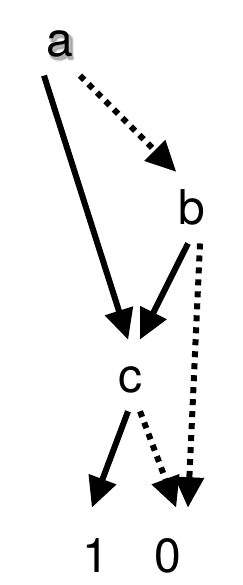
\includegraphics{img/static/dd-dd.png}
\end{span3}
\end{row-fluid}
\end{container-fluid}

\subsection{Decision Diagram 定義}
\label{sec-4-6}

\begin{verbatim}
node :: (index, then, else)
\end{verbatim}

then 枝: index 番目のboolean引数がtrue の時にたどる枝 (1-枝, true枝)

else 枝: index 番目のboolean引数がfalse の時にたどる枝 (0-枝, false枝)

ハッシュテーブルでノードを管理

→同じindex と 子ノード を持つノードは1つしか存在しない (キャッシュされる)

かつ、グラフ上で常にindexが降順で現れる (Ordered DD)

\subsection{関数同士の演算を高速に行える}
\label{sec-4-7}

\begin{container-fluid}
\begin{row-fluid}
\begin{span6}
\begin{itemize}
\item 関数同士の演算(代数系)
\item BDD: $\neg f, f\land g, f\lor g$
\item ZDD: $f \setminus g, f\cap g, f\cup g$
\item ADD: $-f, f\oplus g, f\otimes g, \max (f,g)$
\item コンパクトなまま効率的に計算できる
\end{itemize}
\end{span6}
\begin{span6}
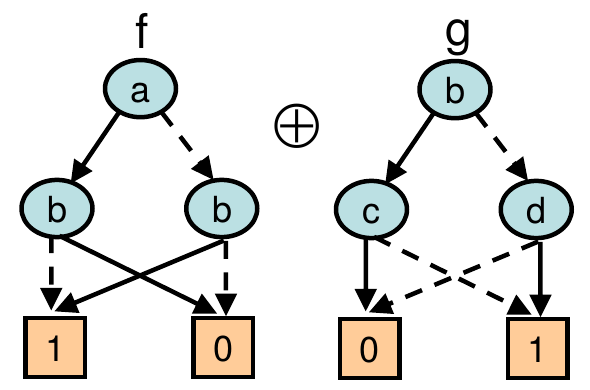
\includegraphics{img/static/dd-operation.png}
\end{span6}
\end{row-fluid}
\end{container-fluid}

\subsection{縮約規則}
\label{sec-4-8}

DD に縮約規則をつけることでさらにコンパクトに出来る

1-枝と0-枝が同じノード を削除 ← 出力に影響を与えない \textbf{無駄なノード} だから

\begin{container-fluid}
\begin{row-fluid}
\begin{span2}

\end{span2}
\begin{span8}
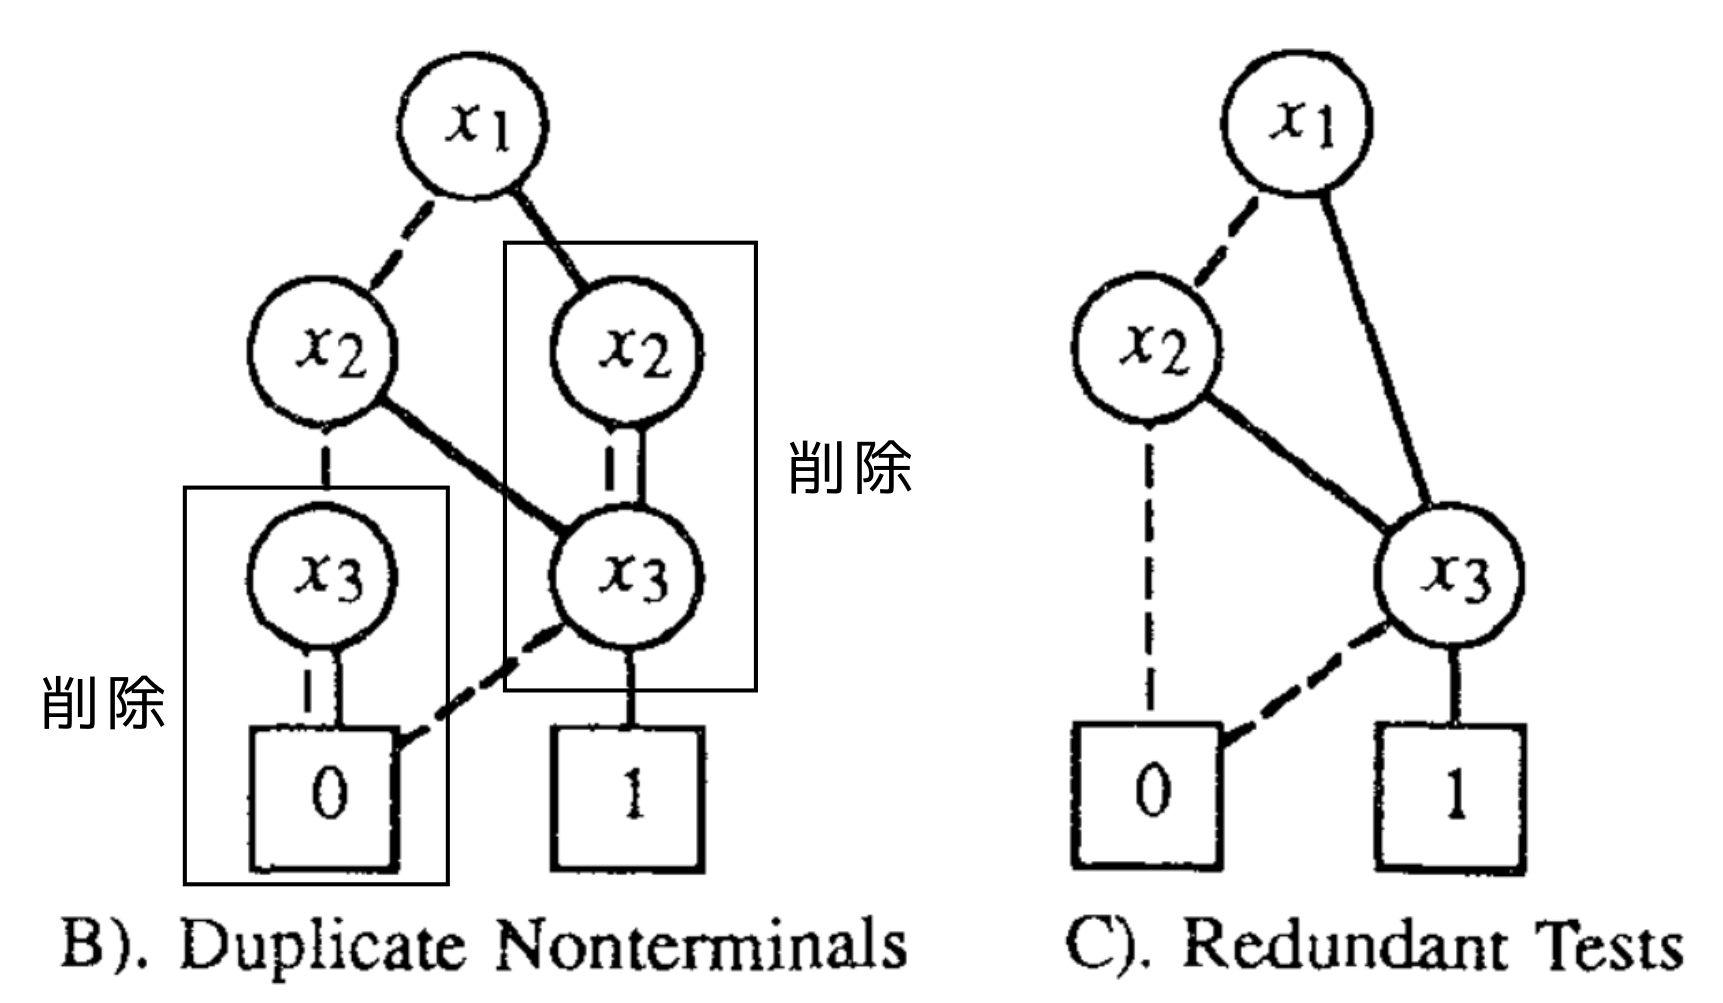
\includegraphics{img/bdd-reduction.png}
\end{span8}
\begin{span2}

\end{span2}
\end{row-fluid}
\end{container-fluid}

正式には \textbf{Ordered BDD (OBDD) == DD + 縮約規則 + 変数順序}

Ordered でないBDDを使うことはまれなので, BDDといえば普通OBDD

\subsection{BDD 同士の演算: Apply}
\label{sec-4-9}

2つのBoolean関数fとgの論理和/論理積などをとることができる

$(f\, R\, g)(x) = f(x)\, R\, g(x),\, x = (x_0,x_1,\ldots)$ のとき ($R=\land,\lor,\ldots$)、

\[
f\, R\, g = \text{BDD}(i,\quad f_{x_i=1}\, R\, g_{x_i=1},\quad f_{x_i=0}\, R\, g_{x_i=0})
\]

ただし $i$ は $f,g$ のルートノードのindex

$f\, R\, g = \text{Apply}(f,g,R)$ と書くと、 Apply は再帰的に定義可能。

\begin{verbatim}
(defun apply (f g op)
  (match* (f g)
    (((bdd index1     then1 else1)
      (bdd (= index1) then2 else2))
     (make-bdd :index index1
	       :then (apply then1 then2 op)
	       :else (apply else1 else2 op)))
    ...(indexが違う場合など)...
    ...(leaf node の場合など)...            ))
\end{verbatim}

\subsection{用途: 自動定理証明、回路の検証、自動プログラム検証 (Formal Methods, Verification)}
\label{sec-4-10}


\begin{container-fluid}
\begin{row-fluid}
\begin{span6}
指数的に多い要素を「並列に」操作できる

→ \textbf{全ケースを余すこと無く検査できる}

注: ここでいう「並列」は、「多数の要素をまとめて処理」ぐらいの意味

並列計算機を走らせることとは関連は無い (が、その意味の並列化も可能)
\end{span6}
\begin{span6}
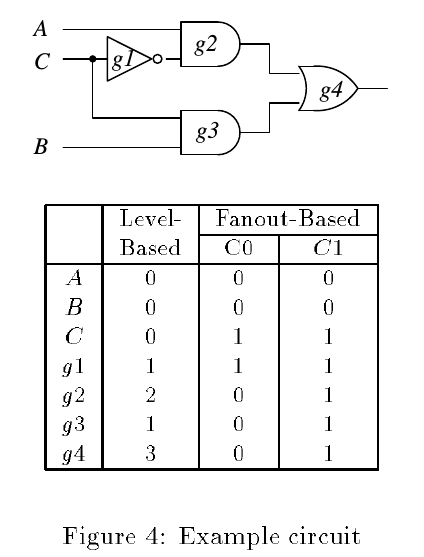
\includegraphics{img/static/circuit.png}
\end{span6}
\end{row-fluid}
\end{container-fluid}

\section{BDDの問題点}
\label{sec-5}

BDD は論理関数を表現するのには良いが、ある種類の関数が得意でない

\textbf{集合族}: $F=\{\{a,b\}, \{a,c\}, \{c\}\}$ --- をBDDで表してみる

関数 $f(x_0,x_1,x_2)$ :

例: $S=\{a,b\}$ は Fに含まれているか?

集合 $S$ が 集合族$F$ に含まれれば $f=1$, 含まれなければ $f=0$

引数 $x_0,x_1,x_2$: 各要素 $a,b,c$ が $S$ に入力に含まれていれば1,含まれていなければ0.

$f(1,1,0) = 1$, 従って $S \in F$

\subsection{実際にやってみると\ldots{}}
\label{sec-5-1}

左は \textbf{いまいち小さくならない} 。

\begin{alignright}
\begin{itemize}
\item → これを改良したのが右の \textbf{ZDD}
\end{itemize}
\end{alignright}

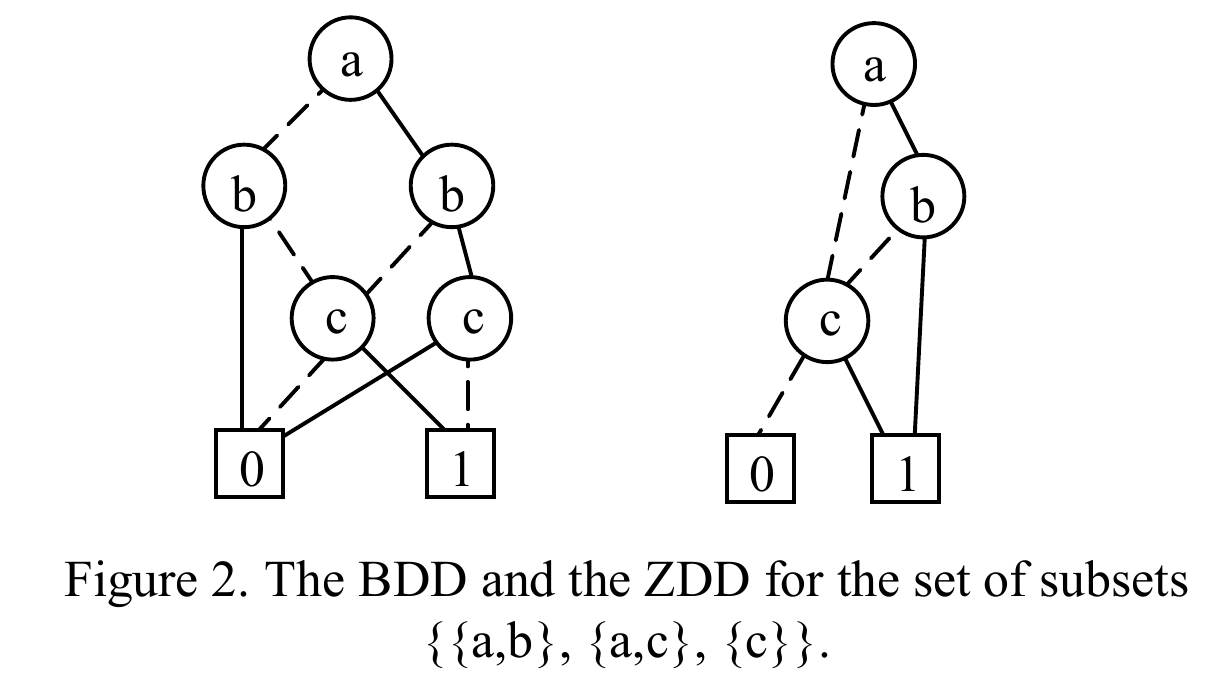
\includegraphics{img/static/bdd-zdd.png}


\subsection{別の縮約規則: Zero-suppressed Decision Diagram (ZDD)}
\label{sec-5-2}

\begin{container-fluid}
\begin{row-fluid}
\begin{span6}
\begin{center}
BDD: 同じなら削除
\end{center}
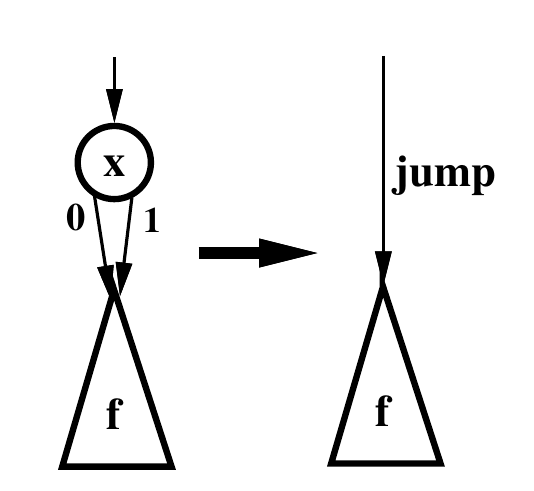
\includegraphics{img/static/reduction-rule-bdd.png}
\end{span6}
\begin{span6}
\begin{center}
ZDD: 1-枝が0なら削除
\end{center}
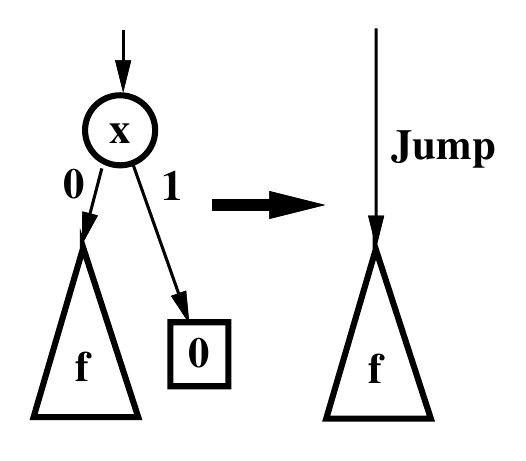
\includegraphics{img/static/reduction-rule-zdd.png}
\end{span6}
\end{row-fluid}
\end{container-fluid}

\subsection{同じ関数でもzddのほうが小さいのは\ldots{}}
\label{sec-5-3}

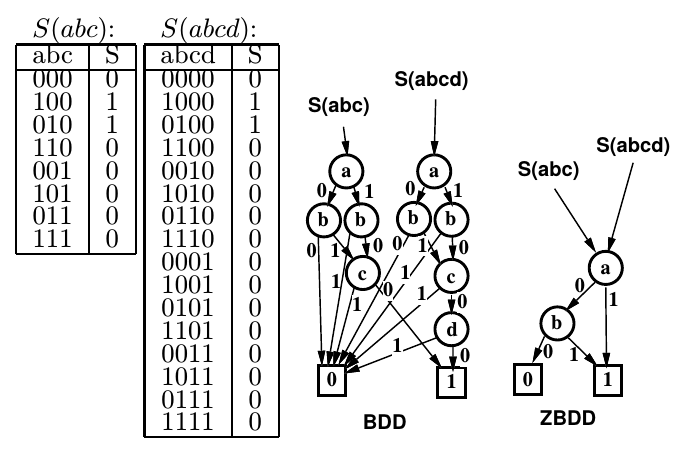
\includegraphics{img/static/bdd-zdd2.png}

\begin{itemize}
\item 理由: \textbf{殆どの場合で関数の値が0} だから
\item → 0と1の割合が同じぐらいの時はbdd, \textbf{0が多い場合にはzddが良い}
\end{itemize}

\section{ZDD は使える}
\label{sec-6}

0が多い場合にはzddが良い

\begin{itemize}
\item \textbf{最悪指数時間の問題を動的計画法で解く場合…}
\begin{itemize}
\item \textbf{空間全体} のうち \textbf{使う空間} はほんの少しなので…
\item 保持すべきデータをzddに貯めれば 殆ど0
\item \textbf{BDD より ZDD が速いはず!}
\item 指数的に速いアルゴリズムを書くのに役立つハズ ≠ 定数倍の高速化
\end{itemize}
\end{itemize}

\subsection{例えば\ldots{} (ERATOのスライドを借用)}
\label{sec-6-1}

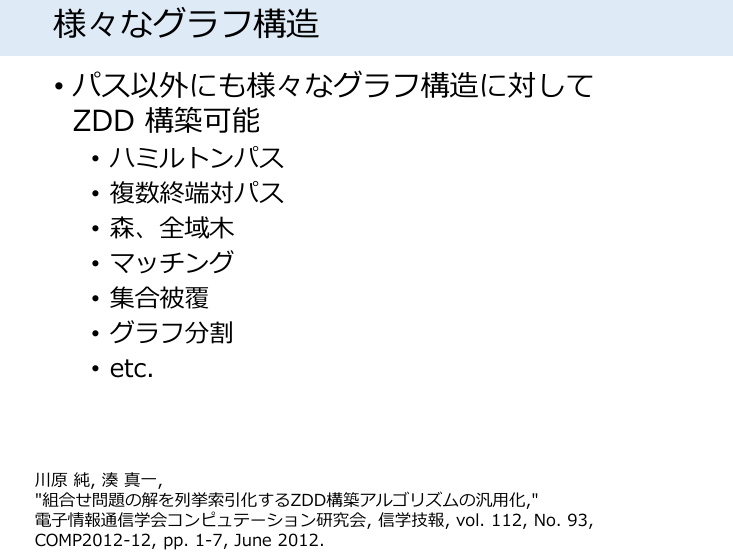
\includegraphics{img/static/graph.png}

\begin{note}
ZDD とフロンティア法 2017年版 ver 0.1 奈良先端科学技術大学院大学 川原 純
\end{note}

\subsection{例えば\ldots{} (ERATOのスライドを借用)}
\label{sec-6-2}

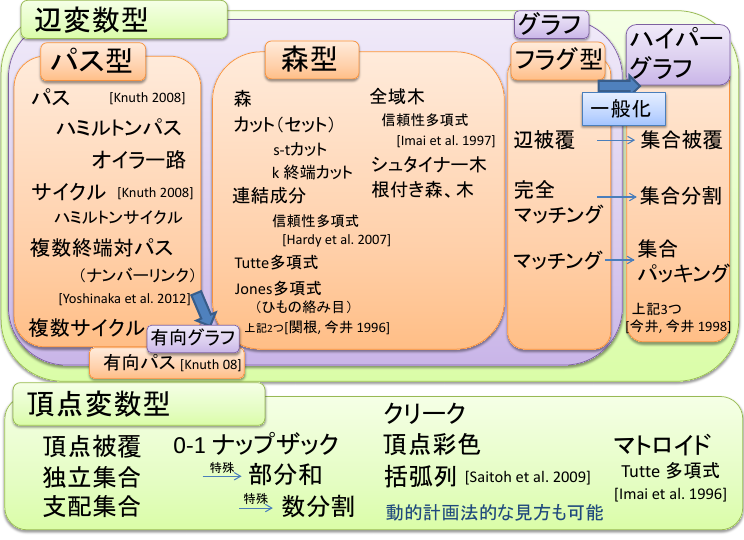
\includegraphics{img/static/graph2.png}

\begin{note}
ZDD とフロンティア法 2017年版 ver 0.1 奈良先端科学技術大学院大学 川原 純
\end{note}

\subsection{例えば\ldots{} (ERATOのスライドを借用)}
\label{sec-6-3}

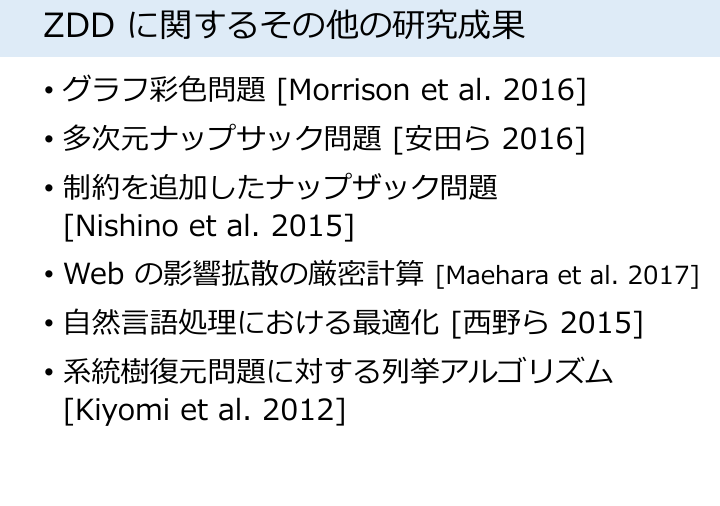
\includegraphics{img/static/graph3.png}

\begin{note}
ZDD とフロンティア法 2017年版 ver 0.1 奈良先端科学技術大学院大学 川原 純
\end{note}

\subsection{例えば\ldots{} (ERATOのスライドを借用)}
\label{sec-6-4}

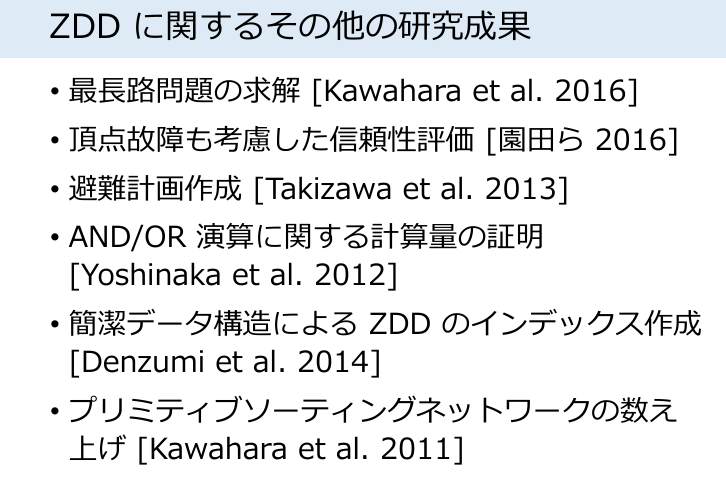
\includegraphics{img/static/graph4.png}

\begin{note}
ZDD とフロンティア法 2017年版 ver 0.1 奈良先端科学技術大学院大学 川原 純
\end{note}

\subsection{ZDDとBDDでは扱うApply操作が違う}
\label{sec-6-5}

BDD: 論理操作 --- $\neg f, f\land g, f\lor g$

ZDD: 集合操作 --- $f \setminus g, f\cap g, f\cup g$

互換性はそこまでではない アルゴリズムも別に作らないといけない

\section{本題: BDD/ZDDをLispから使うためのライブラリ}
\label{sec-7}

BDD は沢山のライブラリがある

\begin{container-fluid}
\begin{row-fluid}
\begin{span3}
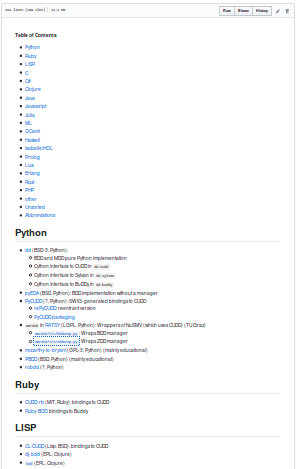
\includegraphics{img/static/bddlib1.png}
\end{span3}
\begin{span3}
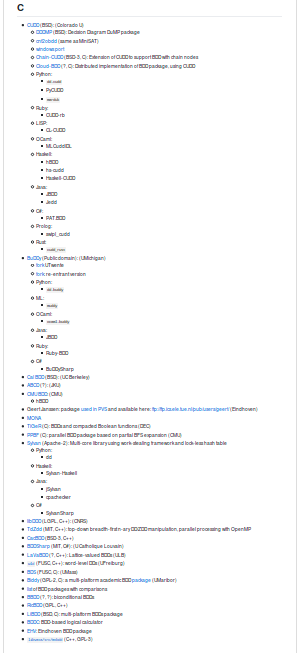
\includegraphics{img/static/bddlib2.png}
\end{span3}
\begin{span3}
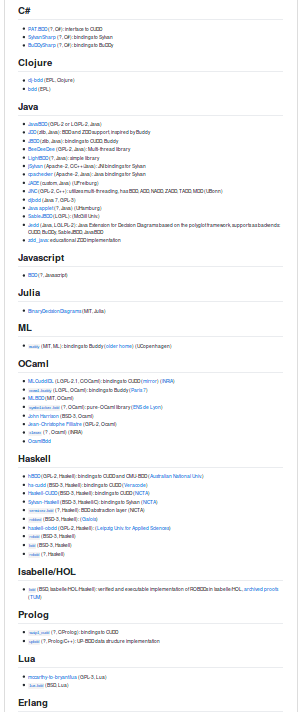
\includegraphics{img/static/bddlib3.png}
\end{span3}
\begin{span3}
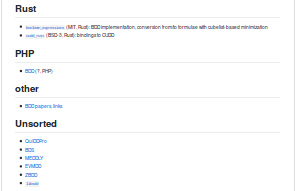
\includegraphics{img/static/bddlib4.png}
\end{span3}
\end{row-fluid}
\end{container-fluid}

\subsection{そのうち、ZDD に対応するのはあまり多くない}
\label{sec-7-1}

\begin{itemize}
\item CUDD: 大御所, Cのライブラリ
\item SapporoBDD, TdZdd (Graphillionの内部): ERATO が作ったC/Pythonライブラリ,
\item ほか数件だけ, つまりZDDはあまりまだ注目されていない

\item CUDD へのCFFIバインディング: CL-CUDD が存在

\item → zdd対応なし, CLOS(遅い), Quicklisp登録なし, テスト無し, Tutorial無し、
CUDDを自分でビルドしてインストールする必要あり, 最新版のCUDDに対応せず。

\item 自分がやったこと: ココらへんを整備して、 \textbf{これで何かを作れることを実証する} こと。
\end{itemize}

\section{Mate-ZDD}
\label{sec-8}

おねえさんのパス数え上げ問題を解くためのアルゴリズム

Don Knuth の Simpath アルゴリズムをピュアZDDで書き直した、シンプルだが遅いバージョン

これをCL-CUDDを使って実装した

\url{https://github.com/guicho271828/simpath}

デモ

\begin{note}
川原 et al. 数理解析研究所講究録 第 1744 巻 2011 年 35-41 ZDD によるパスの列挙
\end{note}

\section{Future Work}
\label{sec-9}

自分の専門である 自動行動計画ソルバ(プランナ)をZDDで作る

\begin{itemize}
\item 配列ベースの普通の手法に比べた利点:
\begin{itemize}
\item よりスケールする(大きな問題が解ける)
\begin{itemize}
\item メモリ使用量が削減できる
\item 探索の情報を圧縮して保持できるから
\end{itemize}
\item \textbf{細かなループの中のチューニングを気にしなくて良い}
\begin{itemize}
\item ZDDが複数の状態をまとめて処理するから
\end{itemize}
\end{itemize}
\end{itemize}

\subsection{BDDベースのプランニングアルゴリズムは存在する:}
\label{sec-9-1}

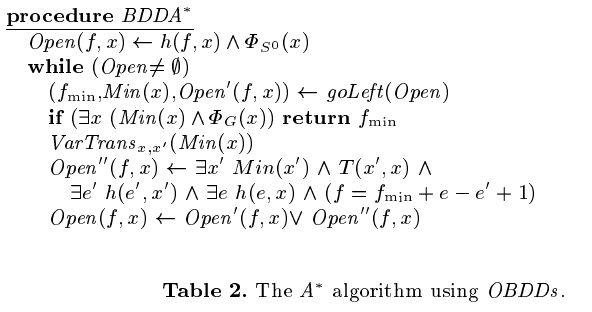
\includegraphics{img/static/bdd-astar.png}

BDDよりZDDのほうがよいハズ

← 指数爆発している全空間に比べ、実際に使われる空間サイズは小さいから

\subsection{International Planning Competition 2014 で優勝}
\label{sec-9-2}

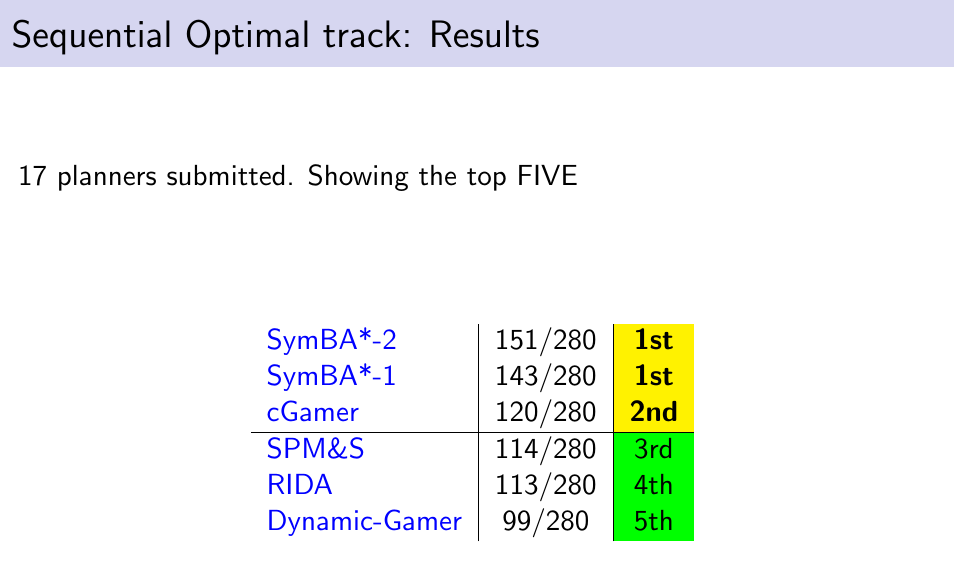
\includegraphics{img/static/bdd-astar-ipc.png}

\subsection{強い}
\label{sec-9-3}


\includegraphics{img/static/bdd-paper1.png}

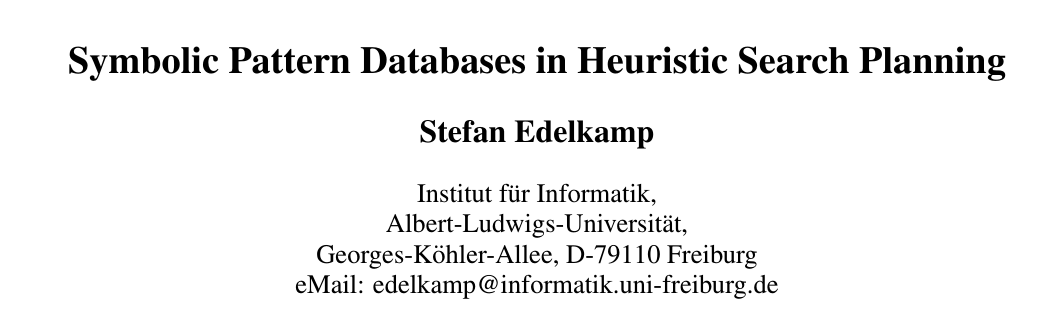
\includegraphics{img/static/bdd-paper2.png}


\begin{alignright}
コレに勝つ!
\end{alignright}

\section{まとめ}
\label{sec-10}

BDD, ZDD を概説

CL-CUDD をまともに使える状態にした

ZDDでお姉さん問題を解くソルバを作った

プランニングに応用したい

\begin{center}
\textbf{\emph{福永研はAIやりたい新規学生募集中! metahack.org}}

\textbf{\emph{Lisper歓迎, 教授もlisper}}
\end{center}
